% !TEX root = ../notes_template.tex
\chapter{Spatio-temporal Models with Seasonal or Multi-year Dynamics} \label{Chap:spatiotemporal}

\section{Monitoring Trends in Abundance and Distribution}

Scientists monitor changes in natural resources, species, or communities over time, and this information is then used by local communities, businesses, and the general public to debate changes in environmental policy and management.  As a few examples:
\begin{itemize}
    \item Voters and legislatures in the United States have defined various state and federal Endangered Species Acts \cite{goble_local_1999}, which outline processes to list plant and animal species as endangered or threatened, and mandate legal protections for those listed species. Criteria for listing include (1) that the species is declining, or (2) that its habitat or range is being damaged or curtailed;

    \item The International Union for Concerned Scientists (IUCN) maintains the IUCN Red List, which identifies which taxa are data-deficient and then assigns other taxa to categories of increasing risk from Least Concern to Critically Endangered, or to different categories for Extinct taxa.  Criteria are evaluated based on evidence of (Criterion A) a decline in population abundance or (Criterion B) a change in area of occupancy \cite{iucn_standards_and_petitions_subcommittee_guidelines_2022}, often based on time-series or spatio-temporal models that infer abundance or habitat utilization \cite{sherley_estimating_2020}; 

    \item Markets exist or are being developed for many types of \myindex{ecological services}.  For example, carbon offset markets seek to attract financial capital for efforts to store carbon and other emissions that would otherwise contribute to global climate change.  The Warsaw Framework for REDD+ established a process to provide global financing for forest management that results in reduced emissions, while also mandating a process to monitor and verify progress and associated uncertainties \cite{pelletier_redd_2013}; 

    \item Non-governmental organizations such as the Marine Stewardship Council establish a process by which commercial products can be certified as sustainable, thereby providing a signal to consumers that can affect product access or price.  These certifications typically involve a process to monitor changes over time, and the success of the certifying standards can itself be assessed by comparing trends for certified vs. non-certified organizations \cite{gutierrez_eco-label_2012}.
\end{itemize}
In general, these examples involve monitoring changes in the total or average value for a system variable over time, and calculating system variables will typically require spatial integration (Section \ref{sec:Chap6_spatial_integration}).  However, it also entails two further challenges.  First, it requires extending our previous spatial models to include spatial variables that change over time.  It also requires defining new system measurements, corresponding to area of occupancy, range edges and other measurements that characterize spatial distribution and dynamics.

\begin{figure}[!ht]
    \caption[Stommel diagram showing variance for spatial and temporal scales]{Stommel diagram showing the hypothesized variance (vertical axis) arising at a given spatial (y-axis) and temporal (x-axis) scale for an idealized marine plankton community, with major biophysical features indicated as letters and labeled on the right-hand side.  Reprinted from \cite{haury_patterns_1978} with permission from SNCSC and available at \url{https://doi.org/10.1007/978-1-4899-2195-6_12}.}
    \centering
    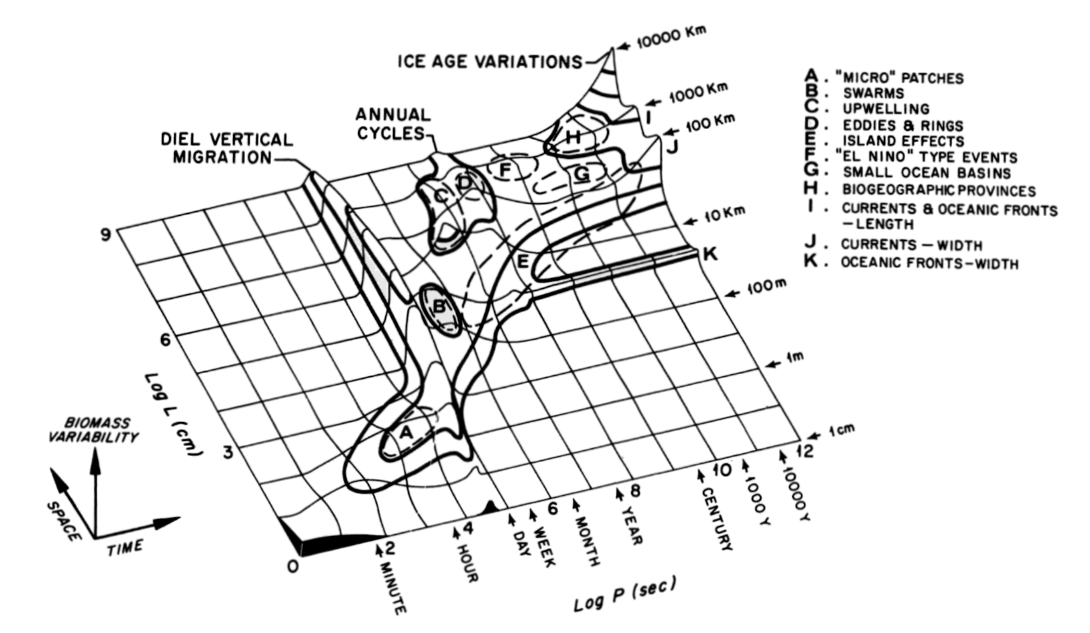
\includegraphics[width=5.5in]{Chap_8/Haury McGowan Wiebe 1978 Fig-1.PNG}
    \label{fig:Chap8_stommel_diagram}
\end{figure}

Complicating matters further, ecological variables have a spatial pattern that varies at a variety of different time-scales.  Important time-scales in ecological systems often include:
\begin{itemize}
    \item \textit{Daily}:  individuals often have daily cycles of higher and lower activity-levels, such that individual tracks will show daily movement between resting and foraging areas.  Similarly, point-count samples of species density will typically show differences in habitat utilization between day and night, including birds or bats returning to rookeries to sleep and the diel vertical migration of zooplankton;

    \item \textit{Seasonal}:  similarly, populations often show predictable cycles in abundance and distribution on seasonal time-scales.  This includes increased vegetation densities in spring and summer, seasonal migrations of mobile consumers, and insects that produce multiple generations per year. Therefore, estimates of habitat utilization may differ between seasons;
    
    \item \textit{Interannual}:  finally, populations often have fluctuations in spatial distribution or total abundance arising over many years.  This includes population cycles for cicadas, years with greater or lesser reproductive output (termed \textit{masting}) for fruiting trees, and population cycles arising from age-structured population and community dynamics.  Therefore, ecological inference about abundance and habitat utilization may differ substantially among years.
\end{itemize}
The magnitude of variation occurring at different spatial and temporal scales is sometimes conceptualized using a \myindex{Stommel diagram} \cite{stommel_varieties_1963}, as popularized in the famous paper \textit{The problem of scale in ecology} \cite{levin_problem_1992}.  For example, inspecting the Stommel diagram for an idealized community of marine plankton \cite{haury_patterns_1978} suggests that daily time-scales have substantial variance across a wide range of spatial scales ranging from 100 m to 100 km (the \textit{Diel vertical migration}), while annual cycles have similar variance on the larger end of this spatial range (Fig. \ref{fig:Chap8_stommel_diagram}).  This approach has been used to identify spatial and temporal scales that are expected to have substantial variance for marine ecosystems in general \cite{hazen_scales_2013}, and could similarly be adapted for use in other ecosystems.

Constructing a spatio-temporal model therefore requires some careful thought regarding how different temporal scales are treated. For example, a model might define a reference level for one time-scale (e.g., estimating summertime habitat utilization and only fitting to summertime samples), integrate across another variable (e.g., including samplings from dawn to dusk and accepting some extra uncertainty arising from differences in distribution between dawn and mid-day behavior) and explicitly estimate differences in another time-scale (i.e., estimating densities occurring in each year).  

\section{Infill and Sprawl Asymptotics}

Despite these different time-scales appearing interchangeably in a Stommel diagram, they have different implications when viewed statistically\footnote{See https://github.com/james-thorson/Spatio-temporal-models-for-ecologists/Chap\_8 for code associated with this chapter.} \cite{cressie_statistics_1993}.  To explain, we first note the distinction between \textit{sprawl and infill asymptotics}.  This distinction applies to designs occurring over space and time, and we provide examples while outlining both below:
\begin{itemize}
    \item \textit{Sprawl asymptotics}\index{sprawl asymptotics} refers to a design where we can increase the spatial or temporal extent but have a fixed density of samples within that extent.  In a time-series design, for example, we may be able to obtain only a single measurement of population abundance in each year.  In this case, we can only increase the amount of data available for statistical inference by extending a study over many years.  As we asymptotically increase the number of years with available data, we will accumulate information about the processes governing changes in abundance over time (parameters representing population dynamics). However, we will never accumulate additional data regarding abundance in any single time.  Intuitively, we might hope to eventually obtain perfect information about parameters but not about state variables;  
    
    \item \textit{Infill asymptotics}\index{infill asymptotics} refers to the opposite case, e.g., when we have a fixed spatial or temporal domain, and can obtain additional samples within that fixed domain but can never sample outside that domain.  In this case, the density of sampling (number of samples per area and/or time) increases asymptotically, and we could theoretically get perfect inference about a state-variable (e.g., population abundance ) within that spatial domain.  By contrast, we cannot obtain samples from locations outside that domain;  this then limits our ability to accumulate information about the underlying relationship between ecological drivers and our target variable (i.e., parameters representing spatial or temporal dynamics).
\end{itemize}
We highlight this distinction because ecologists can often obtain multiple samples at daily and seasonal time-scales (where cyclic drivers occur over a fixed interval), such that infill asymptotics apply at those temporal scales.  However, ecologists who want more information about the relationship between variables at an annual scale must often wait for additional years, such that sprawl asymptotics generally apply at interannual time-scales.  

We further note that spatially correlated random effects can be defined anywhere within a modeled domain.  We can therefore view a sample from a spatial random effect as a realization of a Gaussian process (GP) (see discussion in Section \ref{sec:Chap3_seasonal}), and this GP is sometimes called a \myindex{Gaussian random field} when it is defined over two or more dimensions.  When we can obtain progressively more samples within a fixed domain (such that infill asymptotics apply), we get progressively more and more information about the value of the spatial random effect, and in many cases, we can expect that the estimate will converge on the true value regardless of whether the specified semi-variogram is a good or poor approximation to the true data-generating process.  To make sense of this result, we can invoke a \myindex{representation theorem for Gaussian processes} \cite{klein_representation_1976}, and representation theorems such as this are useful for explaining the asymptotic consistency of estimated mixed-effects models under infill asymptotics.  

As one concrete example, this distinction affects our capacity to estimate parameters governing spatial and temporal autocorrelation.  For example, consider a spatial model fitted to 50 random samples within a 1 square-kilometer spatial domain, in which the true data-generating process follows an exponential correlation function with no measurement error, and we fit the same exponential function to those samples.  We simulate 100 replicates of this experiment, and for each replicate, we use the \colorbox{backcolour}{geoR} package \cite{ribeiro_geor_2022} to first simulate the spatial field, then compute the pairwise difference between each pair of samples and calculate the average difference for different binned distances (i.e., construct a variogram), fit an exponential semi-variance function to these pairwise differences, and compare the estimated semi-variance function against the true (known) semi-variance (see Code \ref{code:Chap8-infill-and-sprawl}).  We specifically compare performance using this original design with two alternative designs, where we either increase sampling density in the same spatial domain (i.e., moving toward performance under infill asymptotics), or a design that increases the spatial area but using the same sampling density per area (i.e., moving toward performance under sprawl asymptotics).  

\lstset{style=Rcode}
\lstinputlisting[language=R, label=code:Chap8-infill-and-sprawl, caption=R code specifying a simulation experiment that compares performance for estimating an exponential semivariance function with either increased sample density or increased sample area., firstline=6, lastline=33, captionpos=t]{Chap_8/Infill_vs_sprawl_asymptotics.R}

\begin{figure}[!ht]
    \caption[Semi-variance estimates with increased sampling density vs. area]{Illustrating performance when estimating an exponential semi-variance in 100 simulation replicates (black lines) compared with the true semi-variance function (blue line), in a design with 50 random samples within a square 1 \(km^2\) spatial domain (left column), or ten times more samples in the same domain along the lines of \textit{infill asymptotics} (500 samples in 1 \(km^2\); middle panel), or ten times more samples over ten times larger area, hence maintaining a constant sampling density along the lines of \textit{sprawl asymptotics} (500 samples in 10 \(km^2\); right panel).  For each design, we also list the percent of replicates where the estimated semi-variance has a geostatistical range beyond the maximum pairwise distance in the original domain, i.e., when the model cannot usefully identify the sill of the semivariance function.}
    \centering
    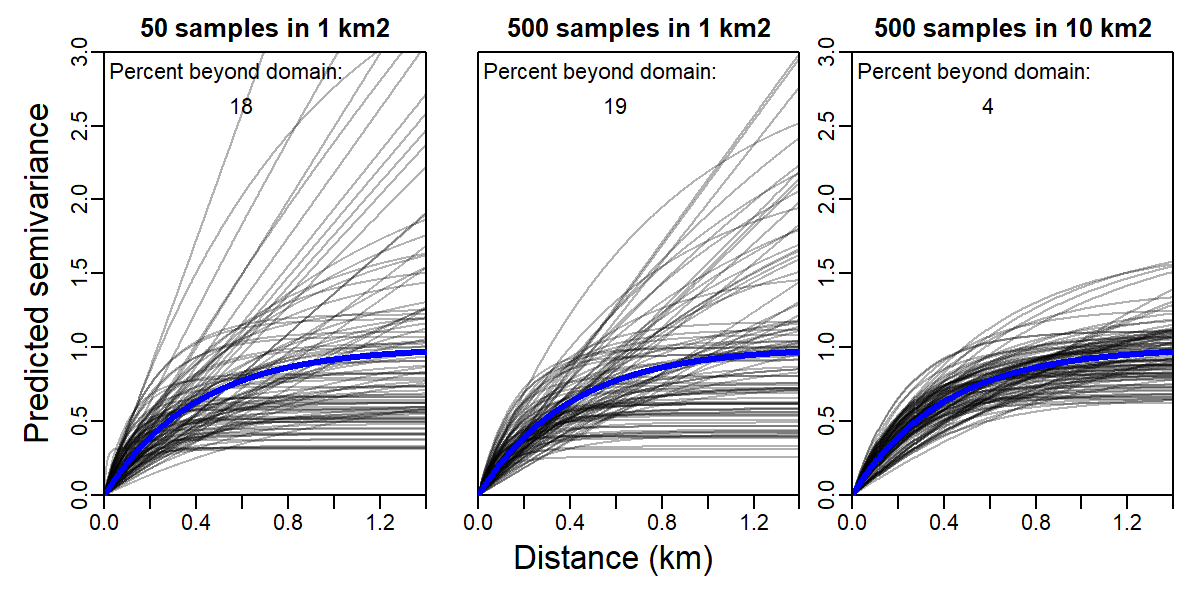
\includegraphics[width=5.5in]{Chap_8/Infill_and_sprawl_asymptotics.png}
    \label{fig:Chap8_infill_and_sprawl}
\end{figure}

Results from this experiment (Fig. \ref{fig:Chap8_infill_and_sprawl}) show that 50 samples over the original domain results in many replicates that cannot identify the variance that occurs as distance increases asymptotically (the \myindex{sill} of the semi-variance function, see Section \ref{sec:Chap3_semivariance}).  These 18 replicates are associated with estimates of the semi-variance function that are essentially straight lines, without any obvious decline in slope for increasing distance.  Perhaps surprisingly, increasing the number of samples by 10-fold within that same domain still results in almost 20\% of replicates that cannot identify the asymptote of the semi-variance function.  However, the same increase in sample size over a larger area (i.e., increasing the area 10-fold while maintaining the original sampling density) results in a large decrease in the replicates that are unable to identify this asymptote.  By contrast, both designs involving 500 samples appear to perform similarly in terms of their ability to estimate the slope at the origin, which corresponds to the predicted rate that variance accumulates per distance for two nearby points.  

This experiment illustrates a few patterns that also typically hold in other circumstances:
\begin{enumerate}
    \item The benefits of increased sampling when estimating parameters for a spatial or temporal model depend greatly on whether the increase arises from increasing sample density (i.e., infill asymptotics) or an increasing domain (i.e., sprawl asymptotics);

    \item To improve performance when estimating parameters (i.e., the correlation across space or time), it is often more helpful to increase the domain being sampled than to increase the sampling density within the existing domain.  In fact, given a fixed domain and infill asymptotics, we might only be able to accurately estimate the rate that variance accumulates per distance (the slope at the origin of the semi-variance function), and not ever have a well-performing estimator of the sill.
\end{enumerate}

And what does this have to do with seasonal vs. inter-annual variation in a spatio-temporal model?  We note that ecologists are often able to wait a year to get a chance to resample habitat utilization within a given season.  Therefore, spatio-temporal variation arising at a seasonal time-scale is likely to have infill asymptotics, and we might hope to eventually accumulate perfect information about seasonal habitat use all else being equal.  However, we can never go back and obtain new samples from the past.  Ecologists must therefore accept that we will often have \myindex{ecological surprise} \cite{doak_understanding_2008} when estimating dynamics over spatial and temporal scales where sprawl asymptotics apply.  

\section{Seasonal Adjustment and Spatially Varying Coefficient Models} 

We next demonstrate different approaches to extend spatial models to include changes in spatial variables over time.  To do so, we extend the analysis from Section \ref{sec:Chap6_spatial_integration}, where we fitted spatial models to ozone concentrations measured on July 1, 2019.  We specifically illustrate how to extend spatial models to account for the daily or seasonal timing of samples by fitting daily ozone concentrations arising from Jan. 1 to Dec. 31, 2019.  But to do so, we first take a detour and discuss seasonal adjustment and spatially varying coefficient models.

\subsection{Seasonal Adjustment}

To address seasonal time-scales, we first introduce the seasonal adjustment for time-series data that is commonly used in econometrics.  For example, an economist might have a time-series of Gross Domestic Product (GDP) \(x_{u,y}\) measured in each quarter \( u \in \{1,2,3,4\} \) and year \(y\).  We use two subscripts for time to highlight the different time-scales involved, but a vector of GPD over time can be extracted as \( \mathrm{vec}(\mathbf X) \).  

GPD has a typical fluctuation during each year, and recessions are typically defined as when GPD shrinks for two consecutive quarters.  However, defining a recession in this way requires first accounting for seasonal fluctuations in GPD, to avoid confusing a recession with a predictable seasonal downturn.  In this case, we can calculate the average difference for GPD in a season relative to GPD in a reference-season, and subtract this difference for each season relative to the reference season \( u^* \):
\begin{equation} \label{eq:Chap8_seasonal_adjustment}
\begin{gathered}
    \bar x_u = \frac{1}{n_y} \sum_{y=1}^{n_y} x_{u,y} \\
    x^*_{u,y} = x_{u,y} - \bar x_u + \bar x_{u^*}
\end{gathered}
\end{equation}
where \(n_u\) is the number of seasons (i.e., \(n_i=4\) using quarterly data), \(n_y\) is the number of years analyzed, and \( \mathrm {vec}(\mathbf X^*) \) is an adjusted measurement of GPD that has removed the average seasonal fluctuations.

We generalize this to define \myindex{spatial seasonal adjustment}. In doing so, we have a few requirements that such an approach must satisfy:
\begin{enumerate}
    \item \textit{Continuous or discrete seasonal timing}:  in Eq. \ref{eq:Chap8_seasonal_adjustment}, we divide the calendar year into a set of discrete seasons (typically quarters or months).  However, ecological data are often collected over a series of weeks, and movement and growth may be substantial during this interval.  We therefore want a generalization of seasonal adjustment that can treat seasonal timing either using discrete seasons, or using a continuous-time process;

    \item \textit{Seasonal correction varies spatially}:  similarly, Eq. \ref{eq:Chap8_seasonal_adjustment} does not include any indexing for location \(s\).  However, seasonal patterns often vary spatially, e.g., where the onset of spring typically occurs later at poleward locations.  We therefore seek a seasonal adjustment method that applies a seasonal-adjustment term that can differ by location.   
\end{enumerate}
Both of these requirements are satisfied using a spatially varying coefficient model involving a cyclic basis spline, which we introduce in subsequent subsections.

\subsection{Spatially Varying Coefficients} \label{sec:Chap8_SVC}

So far, we have discussed generalized linear mixed models with the following form:

\begin{equation}
    g(\mu_i) = \sum_{j=1}^{n_j} x_{i,j} \beta_j + \omega_i
\end{equation}
where \( \mathbf X \) is the design matrix for \(j\) covariates which includes a column of 1s representing the intercept, each covariate has estimated response \( \beta_j \) that is constant across space, and \( \omega_i = \mathbf A_i \omega \) is the value of the residual spatial variable at \(s_i\) given random effects \(\omega\) and projection matrix \(\mathbf A\).  In this model, the spatial variable \( \omega \) can be interpreted as a \myindex{spatially varying intercept}, in the sense that it controls the value of \( \mu_i \) in the absence of covariate effects \( \mathbf x_{i} = \mathbf 0 \).  

As alternative, we next generalize this by introducing \myindex{spatially varying coefficients}, where we include both a spatially varying intercept \(\omega\) but also spatially varying slopes \( \xi \):

\begin{equation}
\begin{gathered}
    g(\mu_i) = \sum_{j=1}^{n_j} x_{i,j} \beta_j + \sum_{k=1}^{n_k} z_{i,k} \mathbf \xi_{i,k} + \omega_i \\
    \xi_k \sim \mathrm {MVN}( \mathbf{0, Q}^{-1} )
\end{gathered}
\end{equation}
where \( \mathbf Z \) is the design matrix with zero-centered spatially varying slopes \( \xi_{i,k} = \mathbf A_i \mathbf \xi_k \). When the same design matrix is supplied for both \(\mathbf X\) and \(\mathbf Z\) then this can be written instead as:

\begin{equation} \label{eq:Chap8_SVC}
    g(\mu_i) = \sum_{j=1}^{n_j} x_{i,j} ( \beta_j + \xi_{i,k} ) + \omega_i
\end{equation}
where it is more obvious that \( \beta_j \) is the spatially averaged response and \( \xi_{i,k} \) the is the local difference relative to this average for covariate \(x_{i,j}\) at location \(s_i\).  Alternatively, there is no reason to require the same covariate matrix for spatially constant and spatially varying slopes. 

Spatially varying coefficient models have been widely used in statistics \cite{gelfand_spatial_2003,hastie_varying-coefficient_1993}, but despite a few exceptions \cite{finley_comparing_2011,thorson_measuring_2019} have seen relatively little use in ecology. Despite this limited use in ecological studies, they could be used to address many common questions including:
\begin{enumerate}
    \item \textit{Local response to regional environmental conditions}: in many cases, an annual index of atmospheric or oceanographic conditions can result in simultaneous responses for species at geographically distant locations (termed an \myindex{ecological teleconnection}).  For example, the wintertime production of sea ice in the Bering Sea drives the spatial extent of cold near-bottom waters in the subsequent spring and summer, and this in turn drives the seasonal migration of demersal fishes.  In this case, it is helpful to include a regional index (summer cold-pool extent) as a covariate with a spatially varying response \cite{thorson_measuring_2019};
    
    \item \textit{Density-dependent habitat selection}:  as a special case of local responses to regional conditions, it may be helpful to specify total population abundance as a covariate and estimate a spatially varying response to this total.  The estimated map of responses then identifies habitats that have a faster- or slower-than-proportional response to changes in total abundance \cite{thorson_development_2022}.  This response-map then approximates the action of density-dependent habitat selection;  
    
    \item \textit{Context-dependent habitat responses}:  alternatively, an analyst might know a priori that two variables have an interactive effect on local densities, but only be able to measure one of the two variables. For example, the importance of predator refuges will likely depend upon the density of predators, which might itself be difficult to measure directly. In this case, the response to the measured variable (predator refuges) is likely to vary among habitats due to the effect of the other missing variable (predator densities).  One short-term response would then be to include predator-refuge as a covariate, and explore the impact of estimating a spatially varying response to this covariate.  Estimates could then be corroborated or refuted by future studies that directly measure the missing covariate;   
    
    \item \textit{Spatially varying detectability}: finally, an ecologist might include sampling gear as an indicator matrix.  For example, if data are available for two sampling gears, then covariate \( z_{i,k} \) would be 0 for the primary gear and 1 for the alternative gear (see Section \ref{sec:Chap7_covariates}).  An analyst might then estimate a spatially varying response to this indicator variable. The spatial response \( \beta_j + \xi_{i,j} \) would then represent the difference in detectability between these two gears at location \(i\).    

\end{enumerate}
Other ecological uses for spatially varying coefficients are reviewed in detail elsewhere \cite{thorson_spatially_2023}.

\begin{figure}[!ht]
    \caption[Periodic spline basis functions]{Illustration of the basis functions resulting from a periodic spline with six degrees of freedom and a period \(T=1\) defined such that the response function has the same value and derivatives at the boundaries \(x=0\) and \(x=1\) (top panel), and ten random simulations of the response function that could arise from using this basis (bottom panel).}
    \centering
    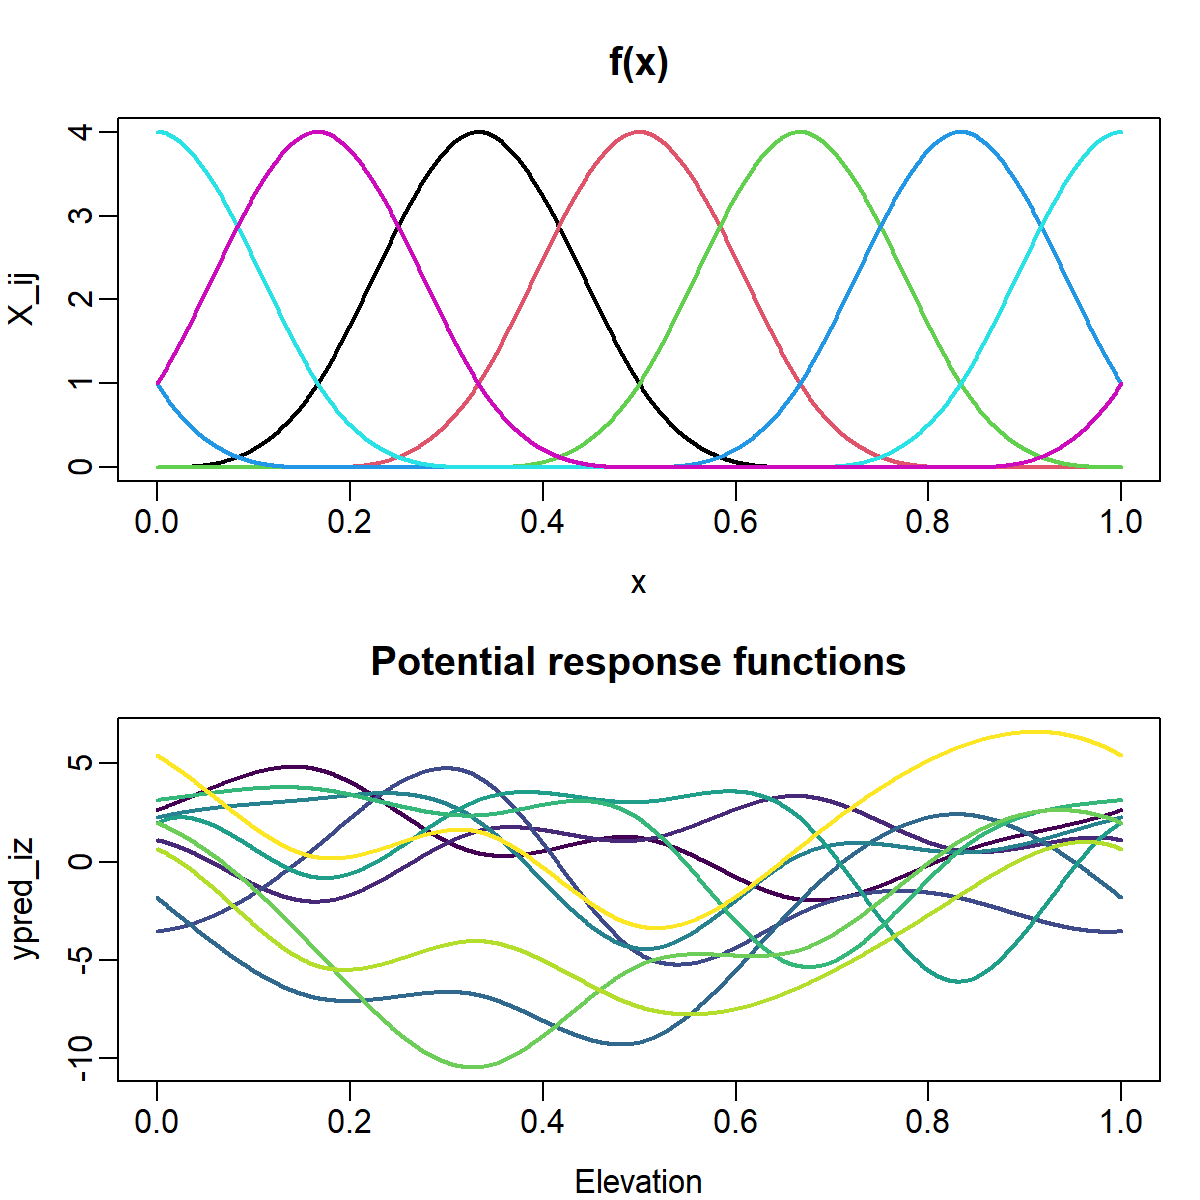
\includegraphics[width=4in]{Chap_6/Basis-cyclic.png}
    \label{fig:Chap8_Basis_cyclic}
\end{figure}

\subsection{Seasonal Spatial Adjustment}

We also previously discussed spline basis-expansion (Section \ref{sec:Chap5:splines}), and how this basis expansion is similar to the basis functions implied by a given spatial correlation function (Section \ref{sec:Chap5_separable_correlation}).  We now extend this by introducing \myindex{periodic splines} (Fig. \ref{fig:Chap8_Basis_cyclic}). A periodic spline specifies that the resulting response function \(f(x)\) has the same value and derivatives at some specified period \(T\), i.e., \( f(x+T) = f(x) \).  For use in seasonal modeling, we can specify a period \( T = 365.24 \) days, such that the response function represents seasonal variation that is repeated every year.  Alternatively, in daily models using high-frequency data, we might specify \( T = 24 \) hours, such that estimated dynamics recur daily. 

\begin{figure}[!ht]
    \caption[Seasonal predictions of ozone concentration in 2019]{Predicted ozone concentrations for each month (with a shared color legend in the bottom-right panel), using a spatially varying response to the periodic spline with six degrees of freedom and a period of 1 year.}
    \centering
    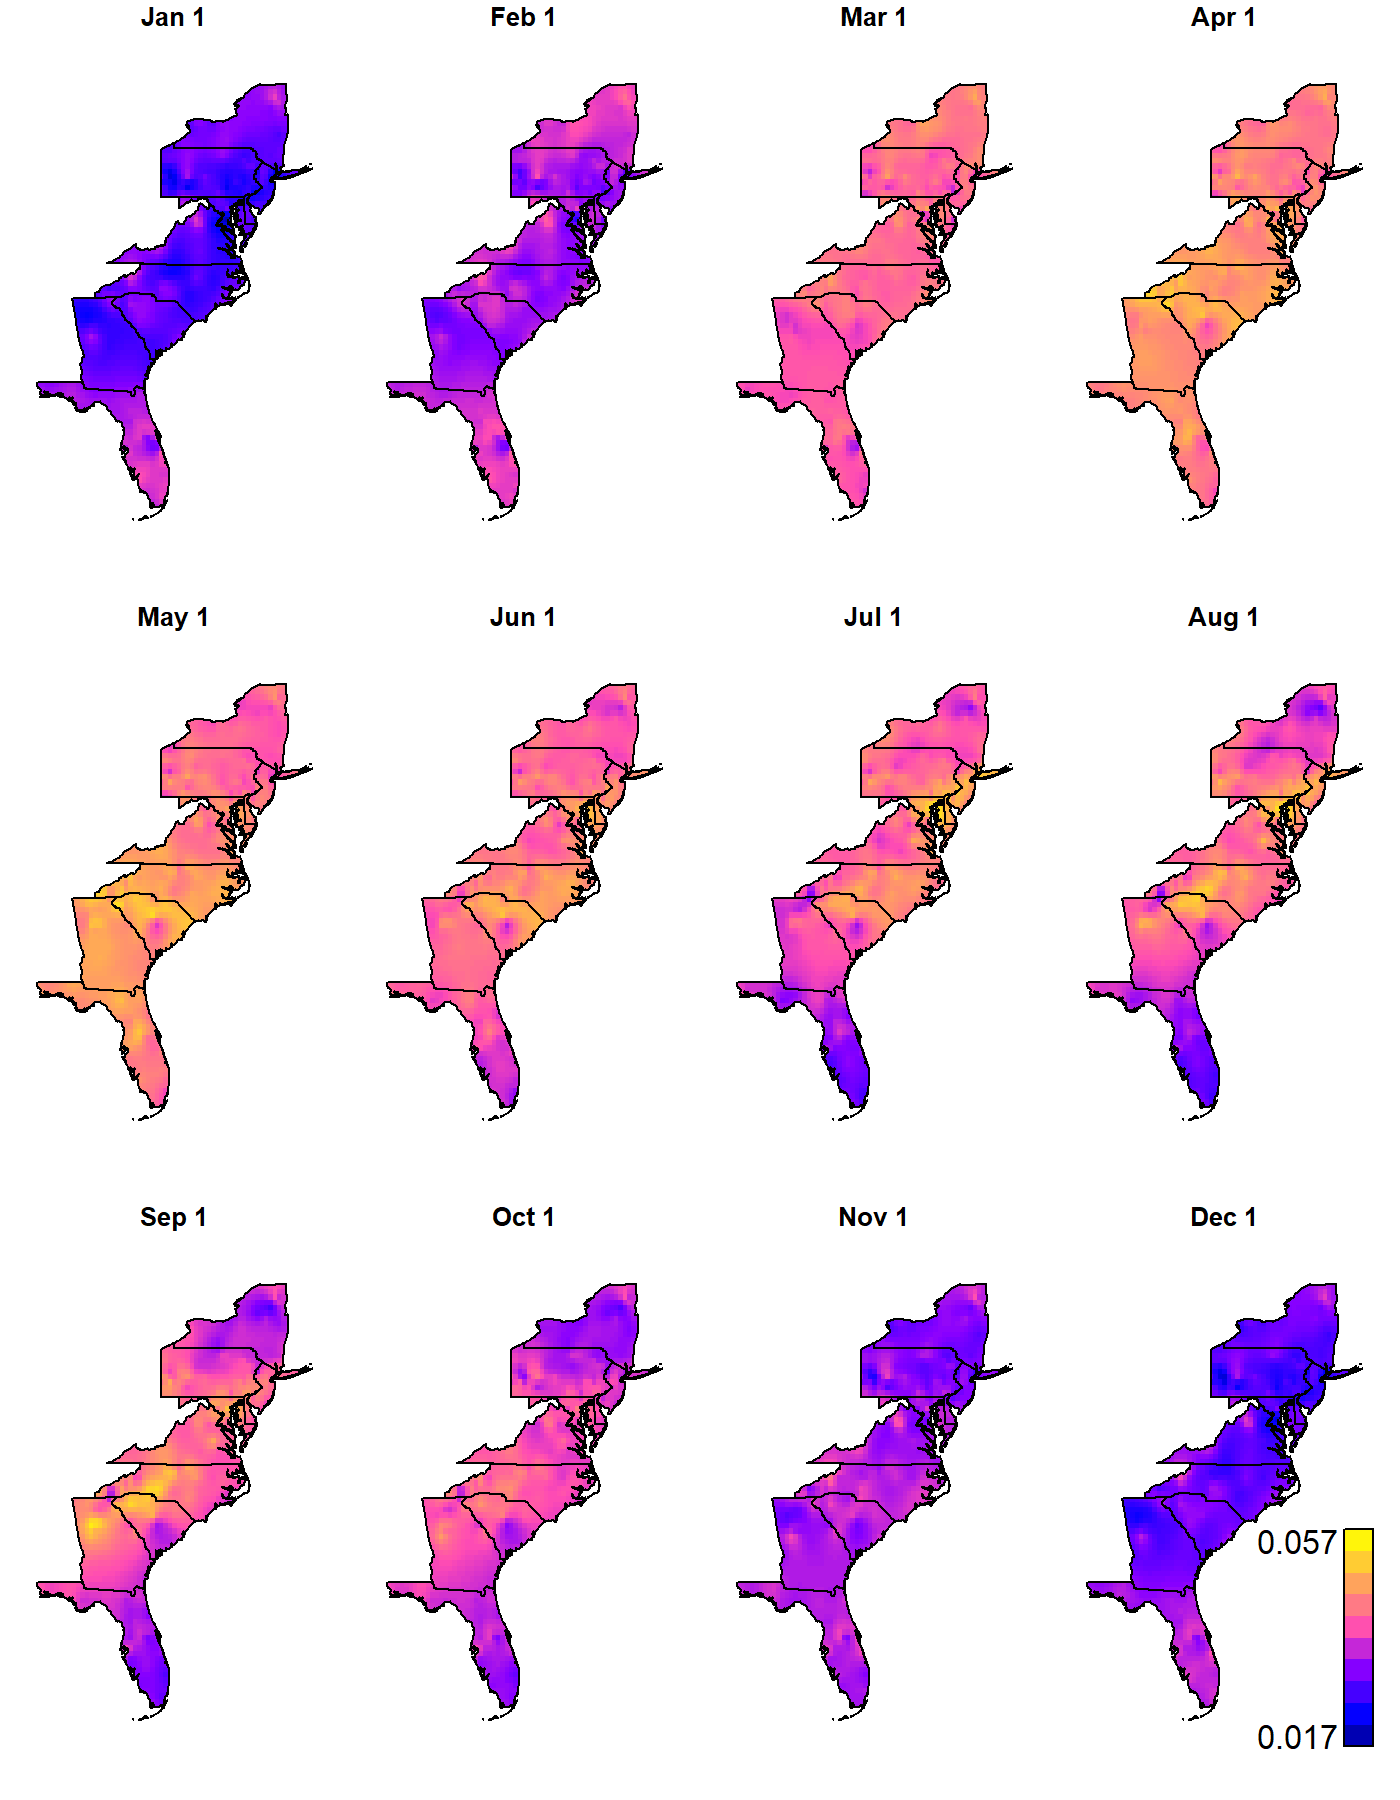
\includegraphics[width=5.5in]{Chap_8/Seasonal_ozone.png}
    \label{fig:Chap8_seasonal_ozone}
\end{figure}

To address seasonal spatial variation, we then include the basis functions resulting from a periodic spline as a covariate in the spatially varying coefficient model (Eq. \ref{eq:Chap8_SVC}). To demonstrate, we specifically fit to 87,520 ozone measurements arising throughout 2019, use six periodic splines with knots distributed evenly throughout the year, and then predict concentrations at the beginning of each month.  Predictions from this seasonal spatial model for July 1 (Fig. \ref{fig:Chap8_seasonal_ozone}) are generally similar to estimates fitted only to data from July 1 (Fig. \ref{fig:Chap6_Mapped_ozone}) in terms of showing lower concentrations in Florida and northern New York and also identifying hotspots along the border between Georgia and South Carolina.  However, they also differ in some cases, e.g., where the seasonal model shows lower concentrations near Atlanta in northern Georgia.  

Importantly, the seasonal spatial model (Fig. \ref{fig:Chap8_seasonal_ozone}) includes only six basis functions with evenly spaced knots but can be mapped for twelve months or at higher temporal frequency. Estimates at high temporal frequency are then interpolated from measurements that are nearby in space and time, e.g., predicted ozone densities on Feb. 1 are intermediate between those estimated for Jan. and March.  Because we use a cyclic spline, this similarity also wraps around the seasonal domain, i.e., where the estimated ozone density in December is similar to Nov. and January.  Infill asymptotics then apply to the estimated seasonal pattern, because we will never need to estimate densities for any season beyond this modeled range. 

\section{Interannual Dynamics} \label{sec:Chap8_interannual_dynamics}

We next outline how to incorporate interannual variation within a spatio-temporal model.  This differs from seasonal variation because interannual variation is likely subject to sprawl asymptotics, while seasonal variation is likely subject to infill asymptotics.  We also outline several different model structures, and which is suitable likely depends upon how the results are being interpreted or used.  

In particular, we introduce different forms of spatio-temporal variation by referring to \textit{main effects and interactions}, to link our discussion to the vocabulary that ecologists use when analyzing experimental data \cite{zuur_mixed_2009}.  We restrict our presentation to \index{separable model}separable models, such that the spatio-temporal covariance \(\mathbf{Q}_{full}^{-1} = \mathbf{Q}_{spatial}^{-1} \otimes \mathbf{Q}_{time}^{-1} \) is formed as the Kronecker product of a spatial covariance \(\mathbf{Q}_{spatial}^{-1}\) and a temporal precision \(\mathbf{Q}_{time}^{-1}\) (see Section \ref{sec:Chap5_separable_correlation}).  We note that there is a large and growing literature regarding \index{non-separable model}non-separable models, where the covariance cannot be constructed as the Kronecker product of smaller processes.  For example, research has developed computationally efficient approaches to construct the spatio-temporal precision resulting from advection and diffusion in atmospheric dynamics \cite{clarotto_spde_2023}.  Some types of non-separable model are simple to specify in TMB, where e.g. a non-separable process can be computed by specifying a first-order Markov process:

\begin{equation} \label{eq:Chap8_nonseparable}
\begin{gathered}
    \mathbf{n}_{t+1} = f(\mathbf{n}_{t}) \times e^{\mathbf{\epsilon}_t} \\
    \mathbf{\epsilon}_t \sim \mathrm{MVN}( \mathbf{0, Q}^{-1} )
\end{gathered}
\end{equation}
where \(\mathbf{n_{t}}\) is a vector of abundance at a set of locations in each time \(t\), \(f(.)\) is a production function that includes nonlinear effects among locations, and \(\mathbf{\epsilon}_t\) is a spatially correlated process error that represents the net effect of exogenous and endogenous drivers that are not included in function \(f\) representing system dynamics.  Specified this way, dynamics \(f\) might include terms representing animal movement, density dependence, and other population-dynamics processes.  This specification extends state-space time-series models (Section \ref{sec:Chap3_Gompertz_model}) by replacing a scalar \(n_t\) representing population abundance with a vector \(\mathbf{n_{t}}\) representing abundance in different areas.  As we saw in Chapters 3 and 5, some (but not all) functions \(f\) could in fact be re-parameterized as a separable model.  Specifying first-order Markov dynamics (Eq. \ref{eq:Chap8_nonseparable}) simply requires computing the probability in each time conditional upon the previous, and this can be computed efficiently even when the resulting dynamics cannot be represented by a separable precision for \(\epsilon\) across all years.   

However, specifying non-separable spatio-temporal models (e.g., applying Eq. \ref{eq:Chap8_nonseparable} directly in TMB code) also has several important drawbacks:
\begin{itemize}
    \item \textit{Slower inner optimizer}:  separable models can often be parameterized such that the inner optimizer can rapidly optimize random effects given the specified value of fixed effects.  By contrast, non-separable models are often harder to parameterize such that the inner optimizer is efficient;

    \item \textit{Decreased sparsity}:  separable models typically maintain any sparsity that is specified for spatial, temporal, or other model dimensions (see Section \ref{sec:Chap5_separable_correlation}).  Without this sparsity, computing the Laplace approximation for non-separable models becomes much slower;  

    \item \textit{Interpretive difficulties}:  separable models can often be explained using a small number of simple concepts.  While this is also true for some non-separable models, it is also possible to specify and fit a non-separable model that is then very difficult to explain or derive from ecological principles.  This lack of simple explanation then results in to difficulties when interpreting outputs, identifying bugs, or comparing results with past research.  
\end{itemize}
We therefore proceed instead by introducing spatio-temporal models using a smaller range of separable specifications, and suggest that these are often worth fitting before exploring nonseparable versions.  In later chapters, we then introduce concepts (e.g., animal movement) that could be useful to include in non-separable spatio-temporal models \cite{thorson_estimating_2021}.  

\subsection{Main Effects for Space and Year}

The simplest model for interannual variation involves calculating a variable as the combination of separate effects for year and location.  For example, we might calculate the density \( d_{s,t} \) using a log-linked linear predictor:

\begin{equation}
\begin{gathered}
  \mathrm{log}( d_{s,t} ) = \beta_t + \omega_s \\
  \mathbf{\omega} \sim \mathrm{MVN}( \mathbf{0, \Sigma} )
\end{gathered}
\end{equation}
where \( \beta_t \) defines the median density in year \(t\) and \( \omega_s \) defines the density for location \(s\) relative to the median location that is typical across years.  This model has several useful properties including:
\begin{enumerate}
    \item \textit{Proportional changes over time}:  for any two years \( t_1 \) and \( t_2 \) the difference \( \beta_{t_2} - \beta_{t_1} \) defines the log-ratio for density at every possible site;

    \item \textit{Rank-order of habitat quality is constant over time}:  the spatial term \( \omega_s \) entirely defines the rank-order of densities across space for a given species.  So for any two sites \( s_1 \) and \( s_2 \), if \( \omega_{s_2} > \omega_{s_1} \) then density will be higher at site \(s_2\) than \(s_1\) regardless of the year being considered; 

    \item \textit{Predictive variance can be low even in areas with no data}:  when predicting density at a location \(s\) and time \(t\), the variance of this prediction only depends upon uncertainty about \(\beta_t\) and \(\omega_s\).  If there is extensive data in a single year \(t_1\) then it is possible to precisely estimate \(\omega_s\).  Then, when predicting density in a new year \(t_2\), all samples are equally informative about \(\beta_{t_2}\) regardless of where those samples occur.  Therefore, predicted density might have a low variance even in an area that is geographically distant from all available data in that year.  
\end{enumerate}
These characteristics cause this \textit{main effects} model to represent a useful null model for thinking about interannual variation in spatial densities.  However, the 3rd property also limits its usefulness in real-world contexts.  

\subsection{Independent Interaction of Space and Time} \label{sec:Chap8_independent_interaction}

Adding complexity progressively, we extend this ``main effects" model for interannual spatial dynamics by using a log-linked linear predictor that includes both spatial and spatio-temporal variation:

\begin{equation}
\begin{gathered} \label{eq:Chap8_spatiotemporal}
  \mathrm{log}( d_{s,t} ) = \beta_t + \omega_s + \epsilon_{s,t} \\
  \mathbf{\omega} \sim \mathrm{MVN}( \mathbf{0}, \sigma_{\omega}^2\mathbf{R}_{\omega} ) \\
  \mathbf{\epsilon}_t \sim \mathrm{MVN}( \mathbf{0}, \sigma_{\epsilon}^2\mathbf{R}_{\epsilon} )
\end{gathered}
\end{equation}
where we have now added a separate spatio-temporal variable \( \mathbf{\epsilon}_t \) for every year, with spatial correlation \(\mathbf{R}_{\epsilon}\) and spatio-temporal variance \(\sigma_{\epsilon}^2\), and these spatial correlation and variance are also specified for the spatial variable \(\mathbf{\omega}\).  This results in the following properties:
\begin{enumerate}
    \item \textit{Spatial differences in habitat quality tend to be preserved}: both \( \omega_s \) and \( \epsilon_{s,t} \) control the relative density for any pair of sites in a given year.  When spatio-temporal variance is smaller than spatial variation, \( \sigma_{\epsilon}^2 << \sigma_{\omega}^2 \), then the relative ranking of densities among sites tends to be preserved over time.  Alternatively, when spatio-temporal variance is bigger \( \sigma_{\epsilon}^2 >> \sigma_{\omega}^2 \), then the relative ranking of densities tends to be scrambled for each pair of years;  

    \item \textit{Areas with no samples in a year tend to have higher predictive variance}:  when predicting densities at a new location using this model, it is necessary to predict the value of both temporal variation \(\beta\), spatial variation \( \omega \) and spatio-temporal variation \( \epsilon \).  To precisely estimate \(\epsilon_{s,t}\) it is then necessary to have data near location \(s\) in that exact year.  Therefore, predictive variance tends to reflect the density of data in that exact time and location.   
\end{enumerate}
For completeness, we note that it is possible to combine these model terms, \( \epsilon^*_{s,t} = \omega_s + \epsilon_{s,t} \).  We can instead form the covariance of that combined term directly as:
\begin{equation}
  \mathrm{vec}(\mathbf{E}^*) \sim \mathrm{MVN}( \mathbf{0, \Sigma}_{\omega} \otimes \mathbf{1} + \mathbf{\Sigma}_{\epsilon} \otimes \mathbf{I} )
\end{equation}
where \(\mathbf{1}\) is a matrix composed of 1s, and \(\mathbf{I}\) is a diagonal matrix.  We can therefore specify \(\epsilon^*_{s,t}\) using a separable covariance (recalling the definition from \ref{sec:Chap5_separable_correlation}).  

\subsection{Autocorrelated Interaction of Space and Time}

Next, we extend the model that includes an interaction of space and time by introducing temporal autocorrelation.  This can include either:
\begin{itemize}
    \item autocorrelation in the temporal main effect, \( \beta_t \); and/or

    \item autocorrelation in the spatio-temporal term \( \epsilon_{s,t} \).
\end{itemize}
Specifically, these involve modifying Eq. \ref{eq:Chap8_spatiotemporal} as:

\begin{equation}
\begin{gathered} \label{eq:Chap8_spatiotemporal_AR}
  \mathrm{log}( d_{s,t} ) = \beta_t + \omega_s + \epsilon_{s,t} \\
  \mathbf{\omega} \sim \mathrm{MVN}( \mathbf{0, \Sigma}_{\omega} ) \\
  \mathbf{\epsilon}_t \sim 
  \begin{cases}
    \mathrm{MVN}\left( \mathbf{0}, \frac{1}{1-\rho_{\epsilon}^2} \mathbf{\Sigma}_{\epsilon} \right) & \text{if } t=1 \\ 
    \mathrm{MVN}( \rho_{\epsilon} \mathbf{\epsilon}_{t-1}, \mathbf{\Sigma}_{\epsilon} ) & \text{if } t>1 
  \end{cases}
\end{gathered}
\end{equation}
where \( \rho_{\epsilon} \) is the magnitude for first-order autocorrelation in spatio-temporal variation, and: 

\begin{equation} \label{eq:Chap8_temporal}
  \beta_t \sim 
  \begin{cases}
    \mathrm{N}\left( 0, \frac{1}{1-\rho_{\beta}^2} \sigma_{\beta}^2 \right) & \text{if } t=1 \\
    \mathrm{N}( \rho_{\beta} \beta_{t-1}, \sigma_{\beta}^2 ) & \text{if } t>1
  \end{cases}
\end{equation}
where \( \rho_{\beta} \) is the magnitude of autocorrelated variation in median density.  In both of these autocorrelated terms, we specify that the variance in the initial year is equal to the stationary variance, which involves correction term \( \frac{1}{1-\rho^2} \) (see below Eq. \ref{eq:Chap3_AR1_stationary}).  However, these autocorrelated terms do not have a stationary distribution when \( \lvert \rho \rvert \geq 1 \), so we would drop the term \( \frac{1}{1-\rho^2} \) if the process approaches a random walk.    

Similar to the previous simplified models, this autocorrelated spatio-temporal model has several useful properties:
\begin{enumerate}
    \item \textit{Density hotspots propagate through time}: when the spatio-temporal term is positively autocorrelated (i.e., \(\rho_{\epsilon} > 0\)), hotspots in density are likely to persist over time.  This then allows for useful interpolation of spatial distribution for years when sampling is not otherwise available \cite{oleary_adapting_2020};
    
    \item \textit{Forecasts converge on a stationary distribution}: similarly, when autocorrelation is within plausible bounds (i.e., \( \lvert \rho_{\epsilon} \rvert < 1 \) and \( \lvert \rho_{\beta} \rvert < 1 \) ), then both \( \beta \) and \( \epsilon \) are stationary and converge on a finite variance (recalling Section \ref{sec:Chap3_semivariance}). In this case, forecasting density from the spatio-temporal model converges on a stationary distribution, which presumably represents the landscape-level variation that is expected over multi-decadal time scales. 
\end{enumerate}
When the autocorrelation terms are set equal, \( \rho = \rho_{\beta} = \rho_{\epsilon} \), this model has been called a \myindex{spatial Gompertz} process \cite{thorson_importance_2014}.  In this case, the value \( 1-\rho \) then measures the strength of density dependence, similar to its role in the conventional Gompertz model (see Section \ref{sec:Chap3_Gompertz}).  

\section{Measuring Changes in Spatial Distribution} \label{sec:Chap8_changes_in_spatial_distribution}

Given this set of models, we can predict density \(d_{s,t}\) across space and among years. To illustrate, we introduce a new case-study, involving walleye pollock (\textit{Gadus chalcogrammus}) in the eastern and northern Bering Sea.  Walleye pollock supports a commercial fishery in the Bering Sea that has a commercial value exceeding 1 billion US dollars annually \cite{bailey_billion-dollar_2013}.  The fishery is operated by a combination of shore-based and at-sea processing facilities, and the catch is frozen to provide low-cost fish worldwide.  The pollock population in the eastern Bering Sea remains one of the most intensively studied fishes worldwide, with a summertime bottom trawl survey in the eastern Bering Sea using an annual fixed station design with approximately 370 stations annually from 1982 to the present day. In recent years, however, the eastern Bering Sea population has expanded northward into areas in the northern Bering Sea, colonizing habitats that were previously too cold for pollock.  The barrier to northward summertime movement is thought to be a body of near-freezing waters near the seafloor, and this \textit{cold pool} is created by ice production near St. Lawrence Island during the preceding winter and spring.  Therefore, a summertime index of ``cold pool extent" is often used to measure bottom-up oceanographic constraints on summertime distribution for this and other species \cite{gruss_synthesis_2021}.  As pollock have moved northward, there has been increased survey effort in the northern Bering Sea.  This ecosystem was previously dominated by an alternative community of Boreal species, and was surveyed following a bottom trawl survey using varied sampling designs (but a consistent sampling gear) in 1982, 1985, 1988, and 1991, and then again in 2010, 2017, 2018, and 2019.   

\begin{figure}[!ht]
    \caption[Pollock density in eastern and northern Bering Sea]{Predicted biomass density (on log-scale; 1st and 3rd columns) and predictive standard deviation for log-density (2nd and 4th columns) in selected years, fitted to annual data for the eastern Bering Sea but only having data in the northern Bering Sea in 1982/1985/1988/1991/2010/2017/2018/2019 (with sample locations shown as bullets on density plots). To improve contrast in plots, we do not plot densities or standard errors (and instead leave those areas white) for any modeled location that has negligible density (defined as \(<0.1\%\) of the maximum estimated density).}
    \centering
    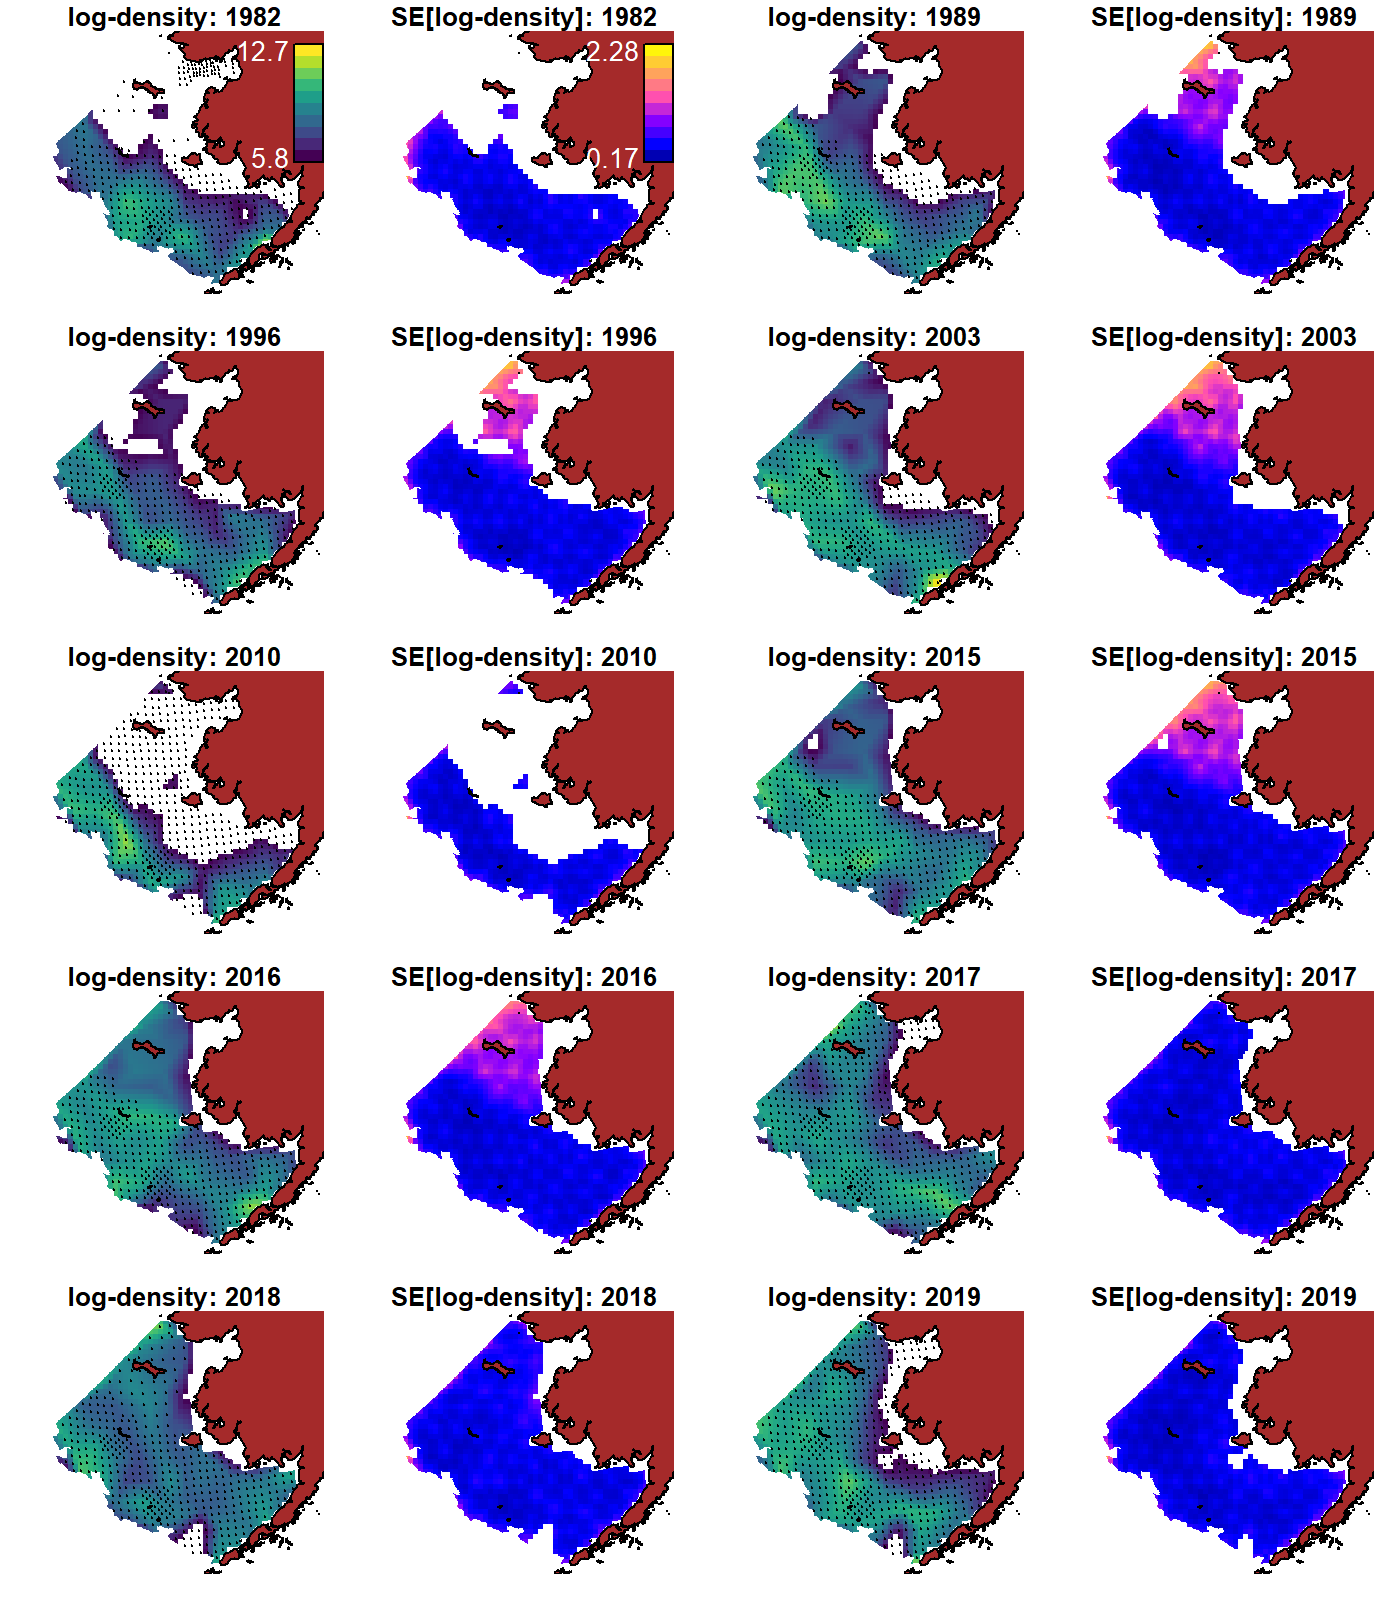
\includegraphics[width=5.5in]{Chap_8/pollock_densities_and_SEs.png}
    \label{fig:Chap8_pollock_densities}
\end{figure}

We fit these data using a Tweedie distribution for survey catches (Eq. \ref{eq:Chap8_spatiotemporal}) and the SPDE methods for spatial correlations. We specify a spatio-temporal model that includes an autocorrelated interaction of space and time (i.e., using Eq. \ref{eq:Chap8_spatiotemporal}) but treating \( \beta_t \) as a vector of fixed effects instead of specifying that it follows an autoregressive process (Eq. \ref{eq:Chap8_temporal}). After fitting, we sample from the joint precision matrix (see Eq. \ref{eq:Chap2_joint_precision}) to visualize predictive uncertainty for density estimates.  Results confirm that predictive standard deviations are low (i.e., 0.2) where data are available in a given year, and are extremely large (i.e., $>$2) in areas without data in a given year.  Similarly, standard errors in the northern Bering Sea in 2016 (i.e., the year before data were available) are lower than in previous years (2014 and 2015) as the variance bridges toward the high precision in 2017 resulting from sampling data in that region (Fig. \ref{fig:Chap8_pollock_densities}).  

\subsection{Indices of Spatio-temporal Dynamics}

We next explore how these predicted densities can be summarized to yield insights about changes in distribution and occupied habitat over time.  As we will see, these methods provide a complementary picture to the estimates of total abundance introduced in Section \ref{sec:Chap6_expansion_weights}.  In addition to the total biomass over the survey domain, we calculate the following metrics:
\begin{itemize}
    \item \textit{Center of gravity}\index{center of gravity}:  for each extrapolation point \(g\) we define some measurement of its spatial position \(z_g\) along some axis.  This measurement could represent geographic location, altitude/depth, or other way of ordering locations along some axis.  We then use this as a covariate in a covariate-weighted average (Section \ref{sec:Chap6_expansion_weights}).  In this example, we define location \(z_g\) as the distance of each point from the equator, and use this to measure poleward shifts in the centroid of the spatial distribution;
    
    \item \textit{{Equivalent area}}\index{equivalent area}:  alternatively, we may seek to measure range expansion/contraction.  This can then be used, e.g., to evaluate whether range size changes during population declines \cite{thorson_density-dependent_2016}.  To do so, we define the \textit{equivalent area} (a.k.a. effective area occupied) as the area necessary to contain the population at its average density \cite{woillez_notes_2009}.  This is then calculated as:
    
\begin{equation}
\begin{gathered}
    B_t = \sum_{g=1}^{n_g} a_g d_{g,t} \\
    D_t = \sum_{g=1}^{n_g} d_{g,t} \frac{a_g d_{g,t}}{B_t}  \\
    A_t = \frac{B_t}{D_t}
\end{gathered}
\end{equation}
    where \( B_t \) is total abundance, \( D_t \) is average density, and equivalent area \(A_t\) is their ratio.  There are many other ways to define area occupied, but this has the benefit that it (1) does not require defining any threshold value to convert estimated densities to some binary presence/absence metric, and (2) it will result in the same value if the spatial configuration of habitats is changed (i.e., it does not depend on occupied habitats being contiguous);
    
    \item \textit{Range edge}\index{range edge}:  finally, we may seek to measure shifts in range edges as an ecological definition of colonizing new habitats \cite{fredston_range_2021}.  To do so, we order extrapolation points based on their location \(z_g\) along some coordinate system, calculate the cumulative sum of abundance along these ordered locations, and identify the location where this cumulative distribution crosses some specified quantile.  For example, we here calculate the poleward range edge as the location where 95\% of population biomass is distributed to the south.  
\end{itemize}
We note that many other metrics can also be calculated where, e.g., the \textit{spreading area} measures range expansion/contraction in a way that is related (but not identical) to the equivalent area presented here \cite{woillez_notes_2009}.  We calculate each of these metrics for each of 500 samples from the joint precision matrix and inspect the resulting time series to infer changes in spatial distribution and population dynamics.  

\begin{figure}[!ht]
    \caption[Measurements of spatial dynamics for pollock]{Measurements of spatio-temporal dynamics for pollock in the eastern and northern Bering Sea from 1982-2019, including total biomass (top-left panel), northward center of gravity (top-right), effective area occupied (bottom-left panel), and northward range edge (bottom-right).}
    \centering
    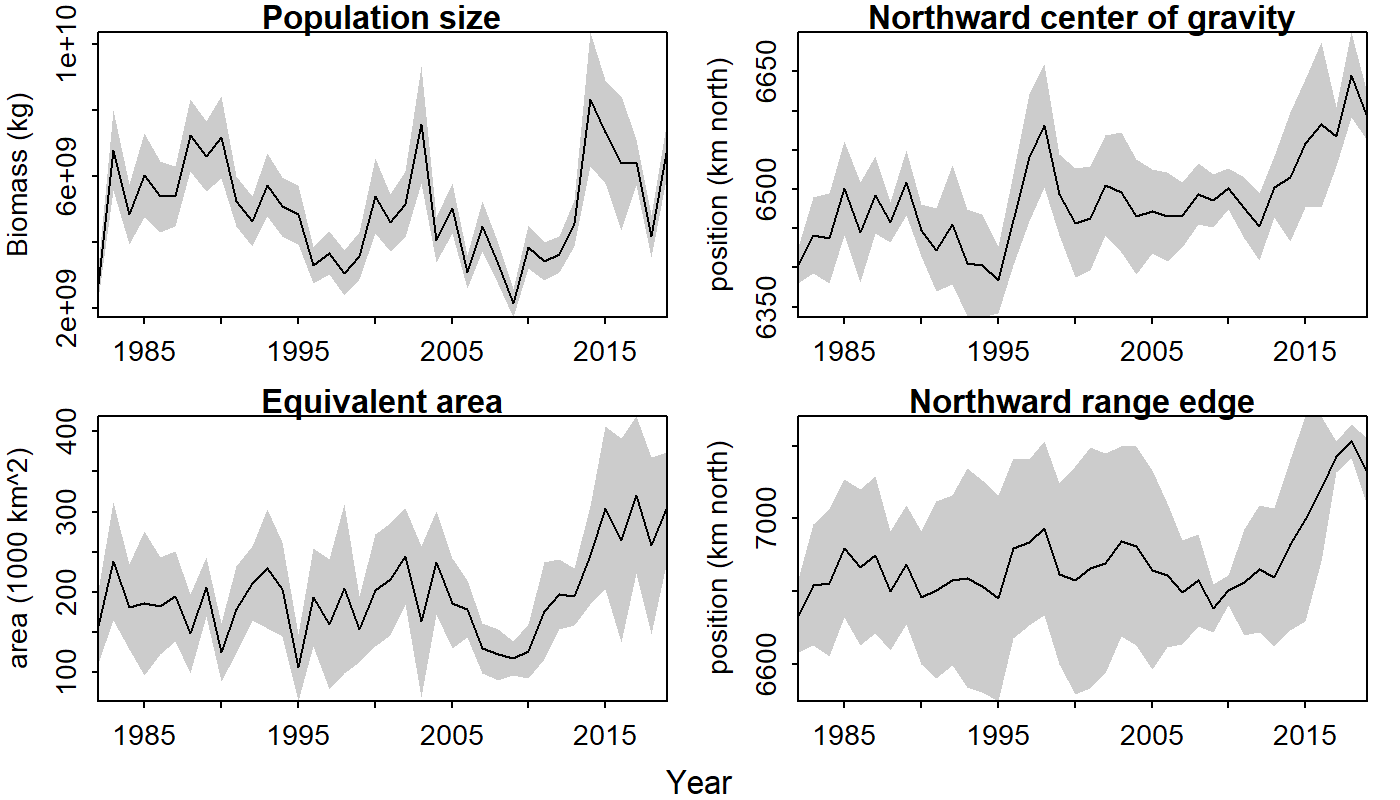
\includegraphics[width=5.5in]{Chap_8/statistics.png}
    \label{fig:Chap8_pollock_timeseries}
\end{figure}

Results for pollock (Fig. \ref{fig:Chap8_pollock_timeseries}) shows that the bottom trawl survey measured available population biomass of 4-8 billion kg from 1982 to 2019, with lowest abundance in 1996--1999 and again 2004--2010.  Importantly, estimated biomass is most imprecise in 2013-2016.  This occurs because the model estimates a substantial density in the northern Bering Sea in 2017, and therefore also expects increasing densities between 2010 and 2017.  However, there is no data to measure this proportion from 2011-2016, so the model compensates by having large standard errors for total biomass in those years.  The estimated center of gravity in 2017--2019 was northward of any previous year, and shifted nearly 150 km from 2015 to 2019.  More dramatically, however, the northward range edge shifted over 400 km north from 2010 (a well-sampled year when the northern range edge was precisely measured) to 2017 (the next year with complete data and therefore a precise estimate of the northward range edge).  This northward range expansion is associated with a dramatic increase in the effective-area occupied from a historical low in 2010 to a high in 2017.  Collectively, these time-series estimates paint a comprehensive picture of a commercially important fish shifting rapidly northwards over time.  

\subsection{Estimating Local Trends}

So far we have shown how to convert output of a spatio-temporal model to time-series that measure changes in spatial attributes for a given population.  However, these do not provide much context for interpreting fine-scale differences in spatial distribution.  We seek a method that summarizes distribution shifts with a level of detail that is intermediate between inspecting density maps for each individual year and reducing these down to individual time-series.

We therefore introduce a method that measures the distance a fish would need to move to maintain a constant population density.  This metric is calculated identically to \myindex{climate velocity} \cite{burrows_ocean_2019,burrows_pace_2011}.  However, climate-velocity is typically applied to a measurement of ocean temperature, and measures the distance that must be moved to keep pace with climate by maintaining a constant temperature.  Our metric is instead intended as a high-level summary of local shifts in distribution, and we therefore call it \myindex{local shifts}.

To calculate local shifts, let's imagine that we have estimated densities \(D(s,t)\) continuously across space and time.  We then define the spatial gradient \( \nabla D(s,t) \), defined as the derivative of the density function with respect to spatial coordinates.  Evaluated at a location \(s\), this results in a vector pointing in the direction of greatest increase in density, with vector length corresponding to the magnitude of that slope, and having units density per distance.  Similarly, we define the temporal gradient \( \frac{d}{dt} D(s,t) \), which indicates whether a location has an increasing or decreasing trend over time with unit density per time.  Finally, we define the local trend as this ratio:

\begin{equation}
  \mathbf{v}(s,t) = \frac{\frac{d}{dt} D(s,t)}{-\nabla D(s,t)}    
\end{equation}
where this results in a vector \( \mathbf{v}(s,t) \) with units distance per time that points in the direction of movement that would be necessary to maintain a constant population density.  

However, we do not actually have a continuous estimate of population density \(D(s,t)\), and instead have discretized this across space and time \(d_{s,t}\).  We therefore replace  derivatives with difference operators.  Specifically, we convert densities at our extrapolation points to values on a grid using the \colorbox{backcolour}{terra} package.  We then use the \colorbox{backcolour}{terra::terrain} function to calculate the spatial slope (i.e., a discretized approximation to the negative spatial gradient \(-\nabla D(s,t)\)), and a series of linear models to calculate a temporal trend (i.e., the discretized approximation to \(\frac{d}{dt} D(s,t)\)) over one or more years.  

\begin{figure}[!ht]
    \caption[Measurements of local trends for pollock from 2010 to 2019]{Visualizing the distance (log kilometers per year) required to maintain a constant population density between 2010 (the year with the smallest equivalent area) and 2019 (after a large expansion northward).}
    \centering
    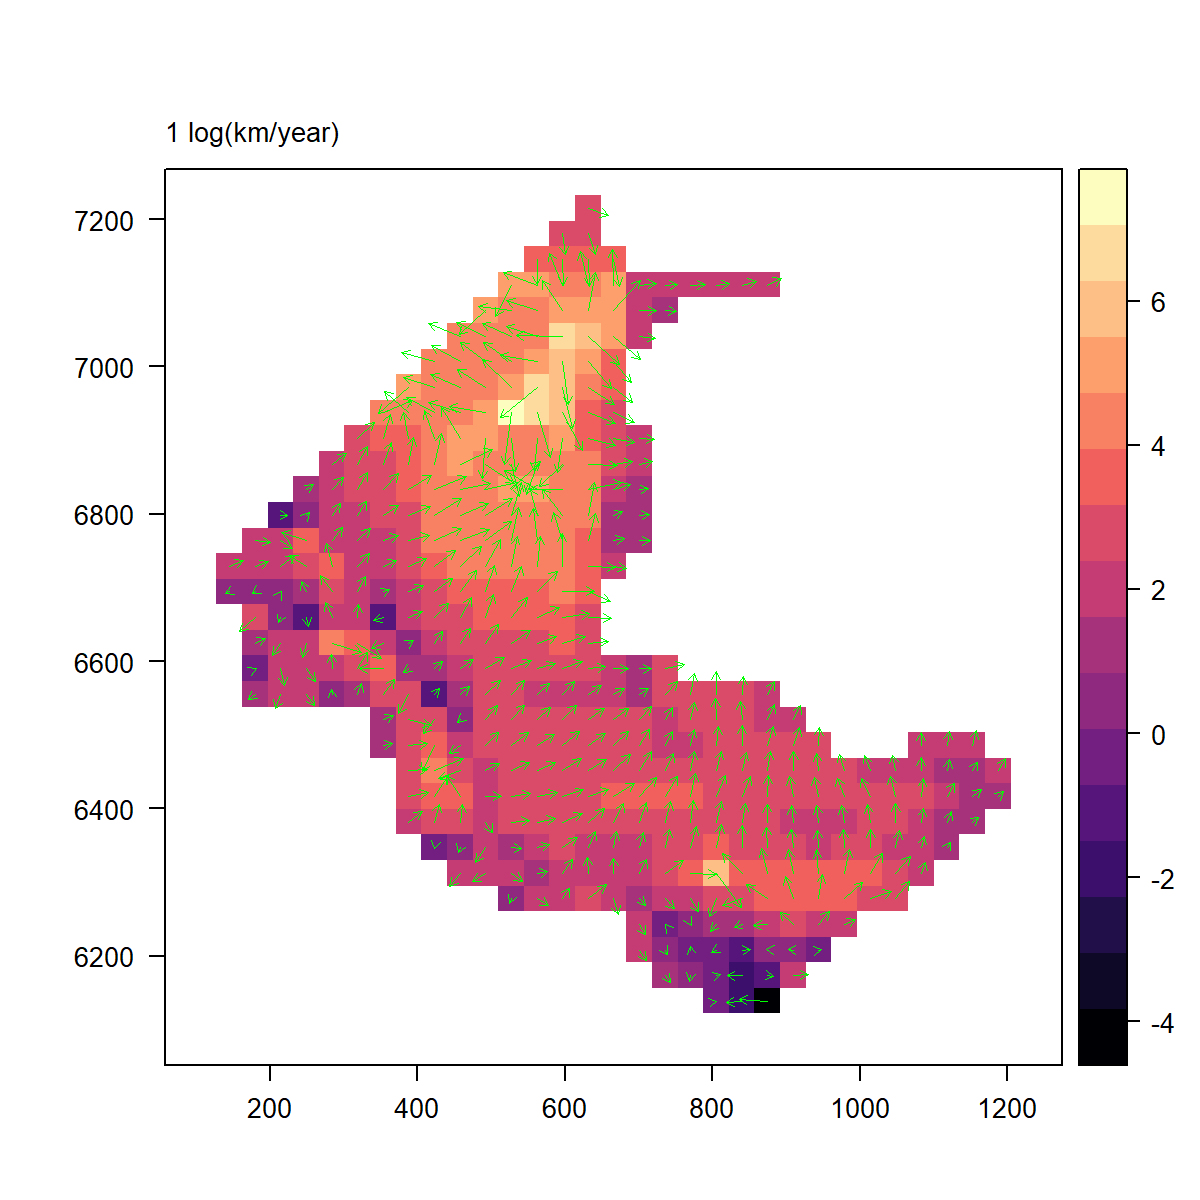
\includegraphics[width=5.5in]{Chap_8/local_trends.png}
    \label{fig:Chap8_local_trends}
\end{figure}

To illustrate the potential for this local-trend calculation, we apply it to estimated log-densities in 2010 and 2019.  These years bookend the rapid shifts northward in both center of gravity and northward range edges, as well as a huge increase in effective area occupied (Fig. \ref{fig:Chap8_pollock_timeseries}).  Inspecting results, we see that locations in the middle and eastern portion of the eastern Bering Sea have trends that require a northeastward movement to maintain a constant density (Fig. \ref{fig:Chap8_local_trends}).  However, local trends are largest and generally point northward in the area between the eastern and northern Bering Seas.  Comparing this local-trends plot with densities in 2010 and 2019 (Fig. \ref{fig:Chap8_pollock_densities}), we confirm that the local-shift metric is a useful depiction of the northward shift in the northern range edge.  

\section{Chapter Summary}

In summary, we have showed that:
\begin{enumerate}
    \item Spatio-temporal dynamics involves variance at a variety of spatial and temporal scales, and dominant scales can be visualized and summarized using a Stommel diagram.  Defining a spatio-temporal model typically involves conditioning results upon a fixed value of some temporal scales (e.g., only using daytime samples to estimate daytime distribution), implicitly averaging across other scales, and explicitly modelling spatio-temporal variation in a selected set of scales;
    
    \item The consequences of increasing sample size depend on whether sampling densities increase within a fixed spatial and temporal domain (i.e., moving toward infill asymptotics) or sampling densities are constant but with increasing spatial or temporal domain (i.e., moving toward sprawl asymptotics).  In particular, sprawl asymptotics is typically necessary to obtain accurate estimates of parameters, while infill asymptotics can improve estimates of state-variables;  
 
    \item Spatially varying coefficient models involve estimating a covariate slope that varies across space.  Infill asymptotics typically apply to estimates of seasonal spatial patterns, and these can be estimated by including a spatially varying coefficient for a periodic spline with an annual period.  The resulting model continuously interpolates the response variable for any season;  

    \item Modeling interannual dynamics in a spatio-temporal model involves some minimal choices about whether to include just the main effect of space and year, or also a space-by-year interaction.  This interaction, in turn, can be independent among years, or autocorrelated to ensure that hotspots are propagated through time;  
 
    \item Spatio-temporal models can be summarized to extract many measurements of shifting habitat utilization, including center-of-gravity, effective area occupied, and range edges. In instances where data are spatially unbalanced, a spatio-temporal model with an autocorrelated space-by-year interaction can appropriately identify an increase in predictive variance for years with spatially restricted sampling.  Spatio-temporal patterns can also be summarized using a metric of local shifts, defined as the direction and distance that an animal would move to maintain a constant population density.  This can then be calculated as the ratio of temporal trend and spatial gradient, and results provide a summary of distribution shifts that is complementary to raw density estimates or high-level time-series summaries.  
\end{enumerate}

\section{Exercise}

\begin{enumerate}
    \item In Section \ref{sec:Chap8_changes_in_spatial_distribution}, we introduced center-of-gravity and range-edge indices as ways to summarize changes in spatial distribution over time.  We then illustrated these by fitting to data for Alaska pollock using an autocorrelated interaction of space and time (Eq. \ref{eq:Chap8_spatiotemporal_AR}).  Please refit this model, but instead using the independent interaction of space and time (Eq. \ref{eq:Chap8_spatiotemporal}) and compare the estimates of spatial indices with those presented in Fig. \ref{fig:Chap8_pollock_timeseries}.  How does it affect the estimates for years with spatially unbalanced sampling (i.e., 2011--2016)?

    \item Continuing this first exercise, please fit the autocorrelated interaction of space and time and add TMB code (e.g., using \colorbox{backblue}{SIMULATE}) to simulate new samples conditional upon the estimates of spatial variables reflecting a progressive northward movement from 2010-2017.  Then refit both the independent (Eq. \ref{eq:Chap8_spatiotemporal}) and autocorrelated (Eq. \ref{eq:Chap8_spatiotemporal_AR}) models.  Do the confidence intervals typically include the true value for spatial indices using both models?  When might you prefer to fit one model or the other?   
\end{enumerate}

